\section*{Chapter 0}
\addcontentsline{toc}{section}{Chapter 0}

\subsection*{0.4}

\begin{figure}[H]
  \centering
  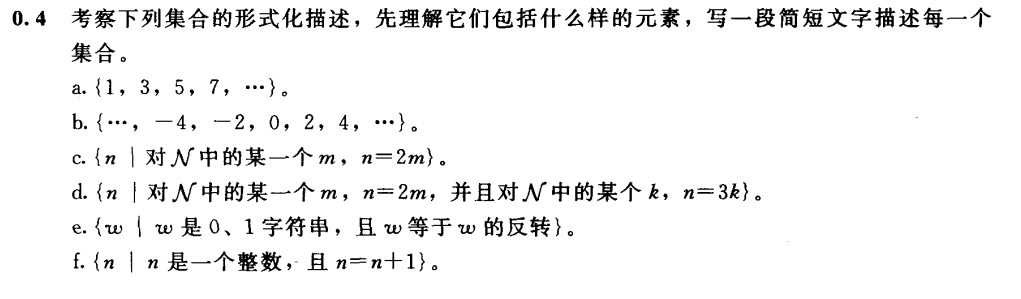
\includegraphics[width=\textwidth]{chapters/imgs/hw_ch0_4.png}
  \caption{}
  \label{fig:hw_ch0_4}
\end{figure}

\paragraph{解答.}
\begin{enumerate}[label=(\alph*), leftmargin=2.5em]
\item 这是所有正奇数组成的集合，即 $1,3,5,7,\dots$。

\item 这是所有偶整数组成的集合，包括负偶数、$0$ 和正偶数。

\item 这是所有能写成 $2m$ 的自然数组成的集合，也就是所有偶自然数。

\item 这是所有同时是 $2$ 的倍数和 $3$ 的倍数的自然数组成的集合，也就是所有 $6$ 的倍数。

\item 这是所有由 $0,1$ 构成并且满足 $w=w^R$ 的字符串组成的集合，也就是所有二进制回文串。

\item 这是空集，因为不存在整数 $n$ 满足 $n=n+1$。
\end{enumerate}

\paragraph{案：}

\subsection*{0.7}

\begin{figure}[H]
  \centering
  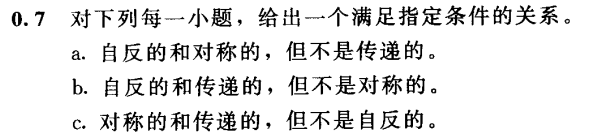
\includegraphics[width=0.7\textwidth]{chapters/imgs/hw_ch0_7.png}
  \caption{}
  \label{fig:hw_ch0_7}
\end{figure}

\paragraph{案：}  可以把关系看成定义在某个顶点集上的一组有向边。这样一来，自反性对应于每个顶点都有一个自环；对称性对应于若存在边 $x \to y$，则也必须存在边 $y \to x$；传递性对应于只要存在
  路径 $x \to y \to z$，就必须再有一条边 $x \to z$。因此，从图的视角来看，这道题实际上是在构造满足若干边性质、但不满足另一些边性质的小型有向图。这个视角对于寻找反例和构造例子都很有帮助。


\subsection*{0.9}

\begin{figure}[H]
  \centering
  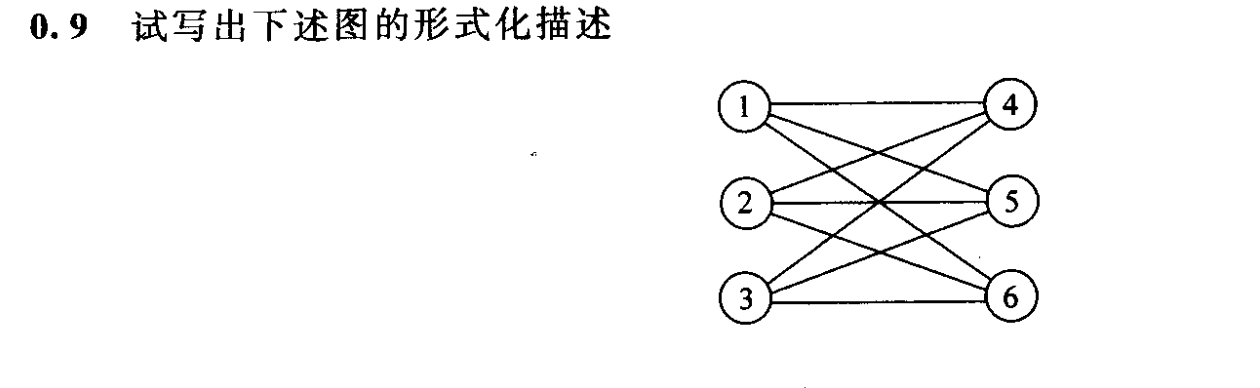
\includegraphics[width=0.7\textwidth]{chapters/imgs/hw_0_9.png}
  \caption{}
  \label{fig:hw_0_9}
\end{figure}

\paragraph{解答.} 
$$
(\{1,2,3,4,5,6\}, \{(1,4), (1,5), (1,6), (2,4),(2,5),(2,6),(3,4),(3,5),(3,6)\})
$$

\paragraph{案：}
图的形式化描述的方法是$(V,E)$，有此约定能通过顶点和边的二元组来形式化描述一个图，同样通过这个约定能从形式化的描述中画出对应的图。

\subsection*{0.10}

\begin{figure}[H]
  \centering
  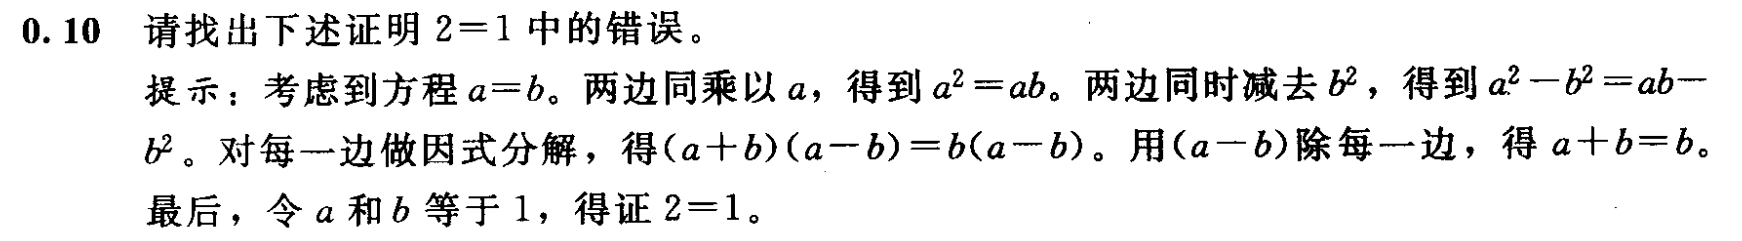
\includegraphics[width=\textwidth]{chapters/imgs/hw_0_10.png}
  \caption{}
  \label{fig:hw_0_10}
\end{figure}

\paragraph{解答.} 

证明 ``$2=1$'' 的错误所在:

原始论证复现

设 $a = b$，则：

\begin{enumerate}
    \item $a = b$（前提）
    \item $a^2 = ab$（两边乘以 $a$）
    \item $a^2 - b^2 = ab - b^2$（两边减去 $b^2$）
    \item $(a+b)(a-b) = b(a-b)$（两边因式分解）
    \item $a+b = b$（两边除以 $(a-b)$） $\longleftarrow$ \textbf{错误在此}
    \item 令 $a = b = 1$，得 $2 = 1$
\end{enumerate}


\textbf{错误出现在第 4 步到第 5 步的推导中。}

由前提 $a = b$，可得：
\[
    a - b = 0
\]

第 5 步的操作是将等式两边同除以 $(a-b)$，即除以 $0$。

\textbf{除以零是未定义的运算。} 在实数域（或任何域）的公理中，乘法逆元的存在性要求：
\[
    \forall\, x \in \mathbb{R},\; x \neq 0 \implies \exists\, x^{-1} \text{ 使得 } x \cdot x^{-1} = 1
\]

当 $x = 0$ 时，不存在这样的逆元。因此，``两边除以 $(a-b)$'' 这一步骤没有合法性，后续一切推导均无效。

\paragraph{案}
该``证明''通过在 $a = b$ 的前提下对 $(a - b) = 0$ 做除法，违反了实数域中\textbf{除法要求除数非零}的基本规则，从而导出了矛盾。错误不在代数变换本身，而在于施加了一个不合法的运算。$\blacksquare$

\subsection*{0.11}


\begin{figure}[H]
  \centering
  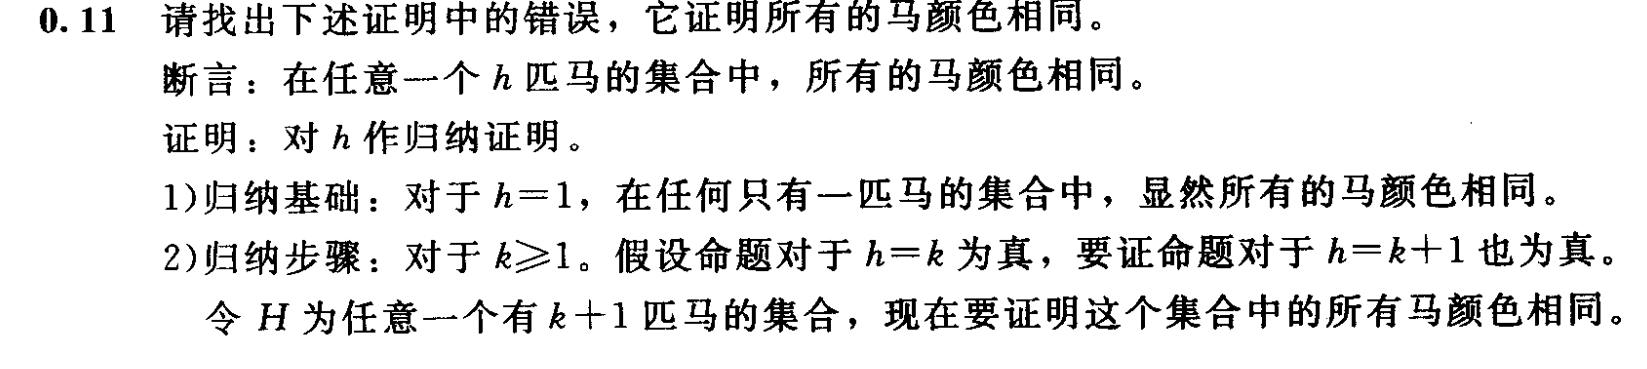
\includegraphics[width=\textwidth]{chapters/imgs/hw_0_11_p1.png}
  \caption{}
  \label{fig:hw_0_11_p1}
\end{figure}

\begin{figure}[H]
  \centering
  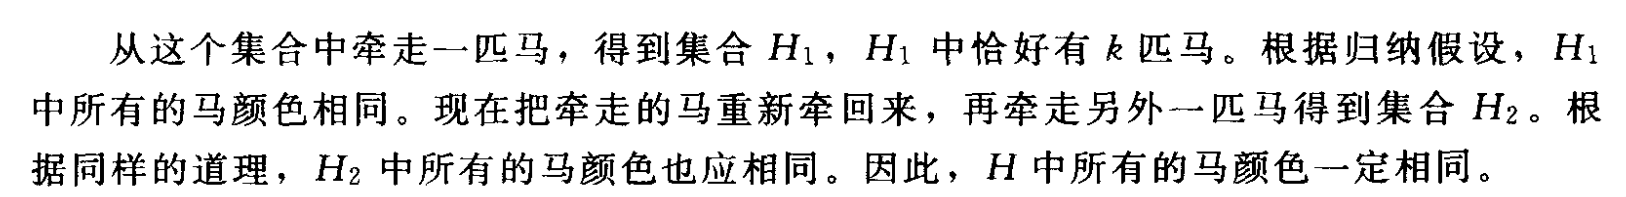
\includegraphics[width=\textwidth]{chapters/imgs/hw_0_11_p2.png}
  \caption{}
  \label{fig:hw_0_11_p2}
\end{figure}

\paragraph{解答.}
\noindent\textbf{\large ``所有马颜色相同''的错误证明——严格分析}

\bigskip

\noindent\textbf{原始论证复现}

\medskip

\noindent\textbf{断言：}在任意一个 $h$ 匹马的集合中，所有的马颜色相同。

\noindent\textbf{``证明''：}对 $h$ 作归纳。

\begin{enumerate}
    \item \textbf{归纳基础：}$h=1$ 时，只有一匹马，显然颜色相同。$\checkmark$

    \item \textbf{归纳步骤：}假设对 $h=k$ 命题为真，证明对 $h=k+1$ 也为真。

    令 $H = \{h_1, h_2, \dots, h_{k+1}\}$ 为任意 $k+1$ 匹马的集合。构造：
    \[
        H_1 = \{h_1, h_2, \dots, h_k\}, \quad H_2 = \{h_2, h_3, \dots, h_{k+1}\}
    \]

    由归纳假设，$H_1$ 中所有马颜色相同，$H_2$ 中所有马颜色相同。

    而 $H_1 \cap H_2 = \{h_2, \dots, h_k\}$ 非空，故 $H_1$ 和 $H_2$ 的马颜色一致，从而 $H$ 中所有马颜色相同。
\end{enumerate}

\bigskip

\noindent\textbf{错误所在}

\medskip

\noindent\textbf{错误出现在归纳步骤从 $k=1$ 到 $k=2$ 的过渡中。}

当 $k=1$ 时，需要证明任意 $k+1=2$ 匹马颜色相同。令 $H=\{h_1, h_2\}$，按上述方法构造：
\[
    H_1 = \{h_1\}, \quad H_2 = \{h_2\}
\]

此时：
\[
    H_1 \cap H_2 = \emptyset
\]

交集为\textbf{空集}。因此无法通过公共元素将 $H_1$ 和 $H_2$ 的颜色``桥接''起来。归纳步骤所依赖的关键推理——

\begin{quote}
    ``$H_1 \cap H_2$ 非空，故两个子集的马颜色一致''
\end{quote}

——在 $k=1$ 时\textbf{不成立}。

\bigskip

\noindent\textbf{严格说明}

\medskip

归纳步骤的论证隐含地使用了如下事实：
\[
    |H_1 \cap H_2| = |H| - 2 = k + 1 - 2 = k - 1
\]

这要求 $k - 1 \geq 1$，即 $k \geq 2$，交集才非空。

因此，归纳步骤仅在 $k \geq 2$ 时有效。而从基础 $h=1$ 到 $h=2$ 的这一步恰好是归纳链断裂的地方——整个归纳证明在最关键的第一步就失败了。

\bigskip

\paragraph{案：}
\medskip

该证明的错误是一个\textbf{归纳步骤的适用范围错误}：归纳步骤要求两个 $k$ 元子集有非空交集（即 $k \geq 2$），但归纳基础仅建立了 $k=1$ 的情形。从 $k=1$ 到 $k=2$ 的推导无法完成，归纳链在起点即断裂。$\blacksquare$


\subsection*{0.13}

\begin{figure}[H]
  \centering
  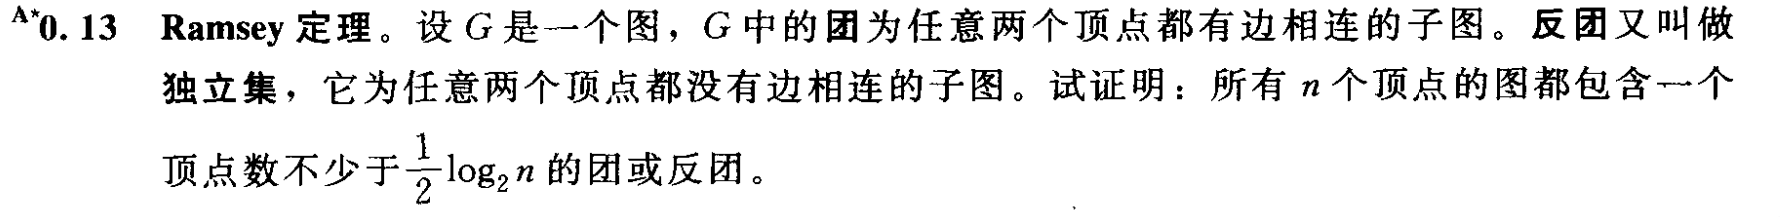
\includegraphics[width=\textwidth]{chapters/imgs/hw_0_13.png}
  \caption{}
  \label{fig:hw_0_13}
\end{figure}

解答:

\begin{figure}[H]
  \centering
  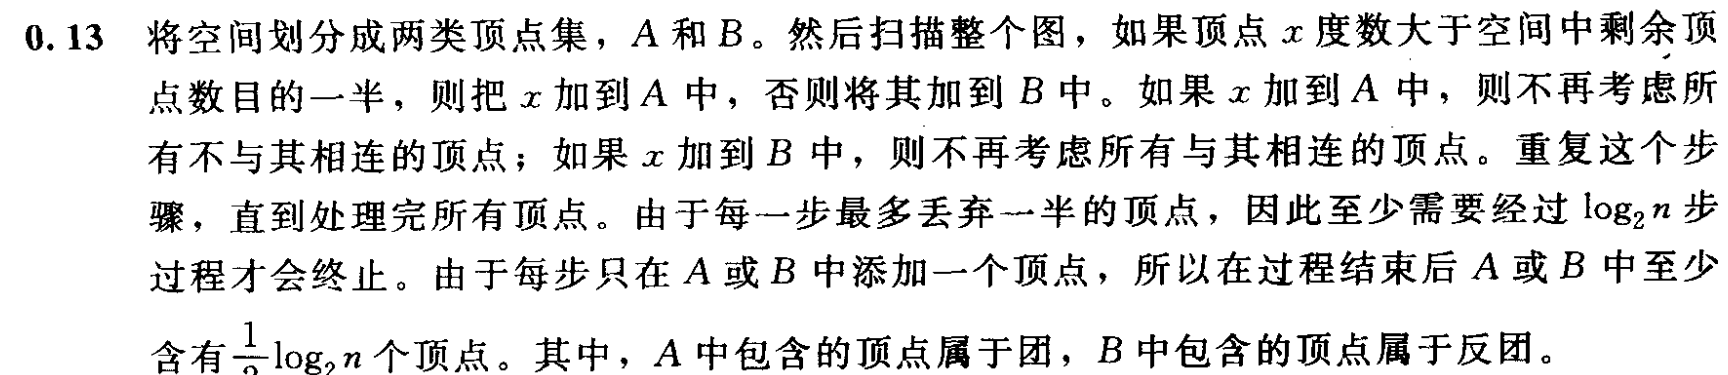
\includegraphics[width=\textwidth]{chapters/imgs/hw_0_13_res.png}
  \caption{}
  \label{fig:hw_0_13_res}
\end{figure}

\paragraph{案：} 这题是通过构造性证明的方式来证明：\textbf{所有n个顶点的图都包含一个顶点数不小于$\frac{1}{2} log_{2}n$ 的团或反团}。通过观察构造出来的算法是如何处理n（节点的个数）证明的这个定理。算法设计用于解决问题，从图灵机的视角来看就是在识别“语言”，回过来分析算法的步骤能得出更多的这个“语言”的性质。如果进一步利用这个性质，或能用于优化这个算法，或能用于优化其他算法。分析做是从另一个视角看一个问题（语言），优化做的是对算法的重新理解。

\clearpage
